\documentclass[UTF8,zihao=5,AutoFakeBold]{ctexart}

\usepackage{graphicx}
\usepackage{subcaption}
\graphicspath{ {images/} }

\usepackage{fontspec}
\setmainfont{Times New Roman}
\setCJKmainfont{Adobe 宋体 Std}
\renewcommand{\baselinestretch}{1.0} % 行距
\ctexset{
    section={
        name={,、},
        number=\chinese{section},
        format = \zihao{3}\bfseries\sffamily\raggedright,
        aftername = {}
    }
}
\usepackage[a4paper,%
left=3.18cm,%
right=3.18cm,%
top=2.54cm,%
bottom=2.54cm%
]{geometry}%
%-------------------------------------------------------------------------------
%	HEADER AND FOOTER
%-------------------------------------------------------------------------------
\usepackage{fancyhdr}  			% use fancyhdr package to get 2-line header
\pagestyle{fancy}\fancyhf{}
\chead{\zihao{-5}《Linux环境程序设计》大作业报告} % Top center head
\cfoot{\thepage}
\renewcommand\headrulewidth{0.5pt} % Size of the header rule

%-------------------------------------------------------------------------------
%	CODE INCLUSION CONFIGURATION
%-------------------------------------------------------------------------------
\usepackage{listings}
\newfontfamily\menlo{Menlo}
\usepackage{color}
\lstset{
    language={[11]C++},
    columns=fixed,
    breaklines=true,
    numbers=left,                                        % 在左侧显示行号
    frame=single,                                        % 显示背景边框
    % backgroundcolor=\color[RGB]{245,245,244},            % 设定背景颜色
    % keywordstyle=\color[RGB]{40,40,255},                 % 设定关键字颜色
    numberstyle=\footnotesize\color{darkgray},           % 设定行号格式
    % commentstyle=\color[RGB]{0,96,96},                   % 设置代码注释的格式
    % stringstyle=\color[RGB]{128,0,0},                    % 设置字符串格式
    showstringspaces=false,                              % 不显示字符串中的空格
    basicstyle=\small\menlo,
    numberstyle=\scriptsize\menlo,
    xleftmargin=0cm,
    xrightmargin=0cm
}
%-------------------------------------------------------------------------------
%	TITLE PAGE
%-------------------------------------------------------------------------------
\newcommand{\titleItem}[1]{\uline{\hspace{\stretch{1}}#1\hspace{\stretch{1}}}}
\renewcommand{\maketitle}{
    \thispagestyle{empty}
    \pagenumbering{gobble}
    \mbox{}
    \vspace{115pt}
    \begin{center} 
        {
            \songti\ziju{0.4}\zihao{-2}
            \addfontfeature{LetterSpace=25}
            \textbf{《} Linux \textbf{环境程序设计》大作业报告}
        }
        \vspace{45pt}

        \zihao{3}\textbf{题目:}\uline{\quad Linux下ls命令的实现\quad}
        \vspace{36pt}

        \zihao{-3}
        \renewcommand{\arraystretch}{1.7} % 行间距
        \renewcommand{\tabcolsep}{0.1cm} % 列间距
        \begin{tabular}{cc}
            学\hspace{\fill}院 & \titleItem{物联网工程学院} \\
            专\hspace{\fill}业 & \titleItem{计算机科学与技术}\\
            班\hspace{\fill}级 & \titleItem{计科1404} \\
            学\hspace{\fill}号 & \titleItem{1030414414} \\
            学生姓名 & \titleItem{阎覃}  
        
        \end{tabular}
        
        \vfill
        \zihao{-2}
        \heiti 二〇一七\songti 年\heiti 十二\songti 月     
        \vspace{20pt}

    \end{center}
}
\usepackage[backend=biber,style=gb7714-2015]{biblatex}
\addbibresource{bibfile.bib}

\usepackage[hidelinks]{hyperref}

\begin{document} 
\maketitle
\newpage

\tableofcontents
\newpage


\pagenumbering{arabic}
\section{设计思想}
本次大作业采用C++编写,运行于Unix/Linux 环境。通过 opendir、readdir、closedir 等函数来操作目录,利用 stat 函数来获取文件信息,完成了一个 Linux 下 ls 命令的程序,并能在Unix/Linux 环境下正确地运行。

最终实现-R、-S、-a、-i、-l、-r、-t、-1这几个选项的功能,即递归查看子目录、按大小排序、显示隐藏文件、显示inode、长格式、倒序显示、按修改时间排序、单列显示。

在设计上尽可能地模仿原版的ls命令,通过man ls命令\cite{LS} 查看原版程序的手册,并且通过亲自试验加强对命令的理解。原版的ls命令有很多细节需要注意,如图\ref{fig:origin_ls}所示,输出的行数会随着终端窗口的宽度自动调整。默认的排序是按照字母顺序排列的,并且是从上到下输出的。所以在编程时要注意输出的排版。每一项最后会添加若干制表符,在终端中每一个制表符的宽度小于等于8个空格,保证最后的输出可以显示最长的文件名。

由于opendir函数不能解析home目录,所以在设计时需要考虑如何获取home目录的路径,替换掉查询中的\lstinline{'~'}字符。

\begin{figure}[h]
    \centering
    \begin{subfigure}[b]{0.4\linewidth}
        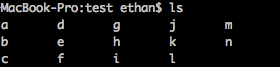
\includegraphics[width=\linewidth]{origin_ls1}
        \caption{宽窗口}
      \end{subfigure}
      \begin{subfigure}[b]{0.3\linewidth}
        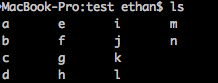
\includegraphics[width=\linewidth]{origin_ls2}
        \caption{窄窗口}
      \end{subfigure}
      \begin{subfigure}[b]{0.7\linewidth}
        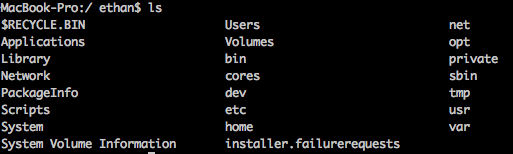
\includegraphics[width=\linewidth]{origin_ls3}
        \caption{每一项用制表符对齐}
      \end{subfigure}
    \caption{原版的ls命令(短格式)}
    \label{fig:origin_ls}
\end{figure}

对于长格式的排版如图\ref{fig:origin_ls_long_format}所示,每列之间用空格隔开,用户名、用户组名、文件名是左对齐,其余右对齐,宽度要可以显示最长的一项。

\begin{figure}[h]
    \centering
    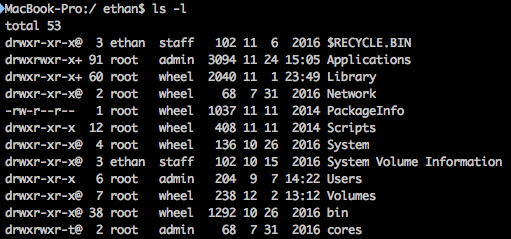
\includegraphics[width=0.7\linewidth]{origin_ls_long_format}
    \caption{原版的ls命令(长格式)}
    \label{fig:origin_ls_long_format}
\end{figure}

\newpage
\section{总体设计}
\subsection{数据定义}

程序主要包含两个类:MyDir和MyFile。

MyDir类表示被查询的所有目录,可以是通过命令行参数传递进来的目录,也可以是递归查询的子目录。类中有两个成员变量:dir和name。其中dir是一个指向DIR的指针,可以通过opendir系统调用得到。name是一个string类型的字符串,保存了目录的路径。这里的路径既可以是相对路径也可以是绝对路径,对于相对路径则始终是相对当前工作目录的路径。

MyFile类表示被查询的所有目录,通过遍历MyDir得到。类中有多个成员变量,包括一个stat类型的成员变量s和多个string类型的输出字段。它有一个构造函数,通过输入所在文件夹的路径和文件名来初始化所有成员变量。它还重载了小于运算符,以便支持排序功能。

程序还有若干全局变量:dirs、options、homeDir、cols。

dirs是一个存放MyDir的栈,它的类型是std::stack<MyDir>。栈顶的元素就是当前需要查询的目录。当查询一个目录时,会将栈顶元素出栈。若开启了递归查询选项,则会将当前查询目录中所有文件夹类型的文件再次入栈。

options是一个整数。利用二进制位来保存程序当前的选项。若开启某一个选项,则将对应的二进位置1。系统支持的选项如图\ref{fig:options}所示。

\begin{figure}[h]
    \begin{lstlisting}
#define LONG_FORMAT     1<<0        // -l
#define INODE           1<<1        // -i
#define SORT_BY_TIME    1<<2        // -t
#define ALL             1<<3        // -a
#define ONE_PER_LINE    1<<4        // -1
#define SORT_BY_SIZE    1<<5        // -S
#define REVERSE         1<<6        // -r
#define RECURSIVE       1<<7        // -R
    \end{lstlisting}
    \caption{配置项的二进制定义}
    \label{fig:options}
\end{figure}
\subsection{系统(函数)调用}

\paragraph{opendir\cite{DIRECTORY}}
打开一个由文件名指定的目录,并且返回一个与其相关的目录流指针。
\begin{lstlisting}[numbers=none]
#include <dirent.h>

DIR *
opendir(const char *filename);
\end{lstlisting}

\paragraph{readdir\cite{DIRECTORY}}
返回一个指向下一个文件的指针。
\begin{lstlisting}[numbers=none]
#include <dirent.h>

struct dirent *
readdir(DIR *dirp);
\end{lstlisting}

\paragraph{closedir\cite{DIRECTORY}}
关闭一个目录流并且释放结构体的内存。
\begin{lstlisting}[numbers=none]
#include <dirent.h>

int
closedir(DIR *dirp);
\end{lstlisting}

\paragraph{getpwuid\cite{GETPWENT}}
根据提供的uid在用户数据库中搜索,返回一个指向passwd结构体的指针,其中包含用户名等信息。
\begin{lstlisting}[numbers=none]
#include <sys/types.h>
#include <pwd.h>
#include <uuid/uuid.h>

struct passwd *
getpwuid(uid_t uid);
\end{lstlisting}

\paragraph{getgrgid\cite{GETGRENT}}
根据提供的gid在用户组数据库中搜索,返回一个指向group结构体的指针,其中包含用户组名称等信息。
\begin{lstlisting}[numbers=none]
#include <grp.h>
#include <uuid/uuid.h>

struct group *
getgrgid(gid_t gid);
\end{lstlisting}

\paragraph{time\cite{TIME}}
返回1970年1月1日0时0分0秒至今的毫秒数。
\begin{lstlisting}[numbers=none]
#include <time.h>

time_t
time(time_t *tloc);
\end{lstlisting}

\paragraph{localtime\cite{CTIME}}
返回一个被转换为本地时间的时间结构体tm,其中包含详细的年,月,日等信息。
\begin{lstlisting}[numbers=none]
#include <time.h>

struct tm *
localtime(const time_t *clock);
\end{lstlisting}

\paragraph{put\_time\cite{put_time}}
按指定的格式格式化时间。
\begin{lstlisting}[numbers=none]
#include <iomanip>

template <class charT>
/*unspecified*/ put_time (const struct tm* tmb, const charT* fmt);
\end{lstlisting}

\paragraph{getenv\cite{GETENV}}
获取环境变量
\begin{lstlisting}[numbers=none]
#include <stdlib.h>

char *
getenv(const char *name);
\end{lstlisting}

\paragraph{ioctl\cite{IOCTL}}
一个专用于设备输入输出操作的系统调用,系统调用的功能完全取决于请求码。
\begin{lstlisting}[numbers=none]
#include <sys/ioctl.h>

int
ioctl(int fildes, unsigned long request, ...);
\end{lstlisting}
\newpage
\subsection{处理流程}

系统的流程图如图\ref{fig:flowchart}所示。首先系统会对输入的所有参数进行处理,对于以'-'开头的字符串,将会被识别为选项。若处理完全部选项则将剩余的作为待查询目录,放入堆栈。之后对栈顶元素进行出栈,遍历此目录。若开启了递归遍历选项则将此目录中所有文件夹再次入栈。遍历完一个目录后再按照格式对所有文件进行输出。重复以上操作直到栈为空,程序结束。

\begin{figure}[h]
    \centering
    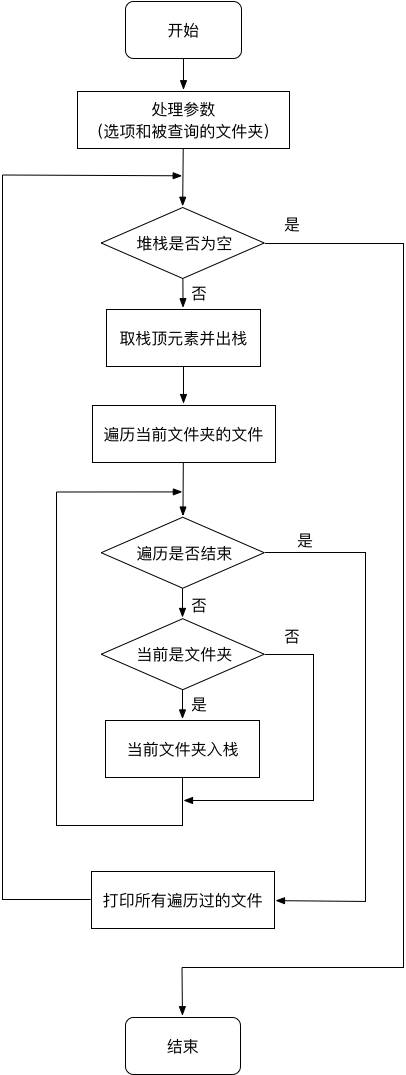
\includegraphics[width=0.4\linewidth]{流程图}
    \caption{系统流程图}
    \label{fig:flowchart}
\end{figure}

\newpage
\section{详细设计(含源程序)}
\lstinputlisting{../src/main.cpp}

\newpage
\section{运行结果与分析}

如图\ref{fig:myls_and_ls}所示,本程序的排版和linux系统自带的ls命令差别不大。

\begin{figure}[h]
    \centering
    \begin{subfigure}[b]{0.7\linewidth}
        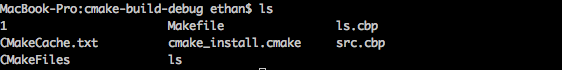
\includegraphics[width=\linewidth]{ls}
        \caption{系统的ls命令}
      \end{subfigure}
      \begin{subfigure}[b]{0.7\linewidth}
        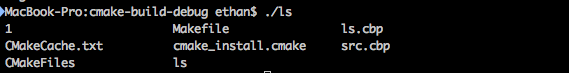
\includegraphics[width=\linewidth]{myls}
        \caption{本程序}
      \end{subfigure}
    \caption{本程序和系统的ls命令对比}
    \label{fig:myls_and_ls}
\end{figure}

如图\ref{fig:myls_and_ls_error}所示,当输入的文件名出错时,会有相应的错误提示。
\begin{figure}[h]
    \centering
    \begin{subfigure}[b]{0.7\linewidth}
        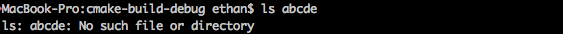
\includegraphics[width=\linewidth]{ls-error}
        \caption{系统的ls命令}
      \end{subfigure}
      \begin{subfigure}[b]{0.7\linewidth}
        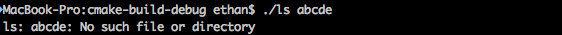
\includegraphics[width=\linewidth]{myls-error}
        \caption{本程序}
      \end{subfigure}
    \caption{本程序和系统的ls命令对比(文件名错误)}
    \label{fig:myls_and_ls_error}
\end{figure}

如图\ref{fig:myls_and_ls_usage}所示,当输入的选项错误时,会有用法提示。
\begin{figure}[h]
    \centering
    \begin{subfigure}[b]{0.7\linewidth}
        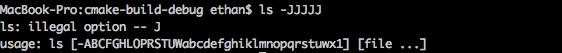
\includegraphics[width=\linewidth]{ls-usage}
        \caption{系统的ls命令}
      \end{subfigure}
      \begin{subfigure}[b]{0.7\linewidth}
        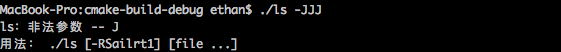
\includegraphics[width=\linewidth]{myls-usage}
        \caption{本程序}
      \end{subfigure}
    \caption{本程序和系统的ls命令对比(选项错误)}
    \label{fig:myls_and_ls_usage}
\end{figure}

如图\ref{fig:myls_and_ls_R}所示,开启递归选项('-R')时,会按照深度优先的方式递归搜索所有子文件夹。
\begin{figure}[h!]
    \centering
    \begin{subfigure}[b]{0.4\linewidth}
        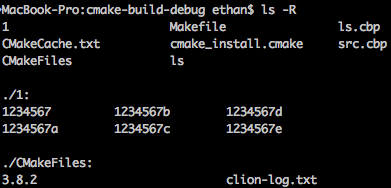
\includegraphics[width=\linewidth]{ls-R}
        \caption{系统的ls命令}
      \end{subfigure}
      \begin{subfigure}[b]{0.4\linewidth}
        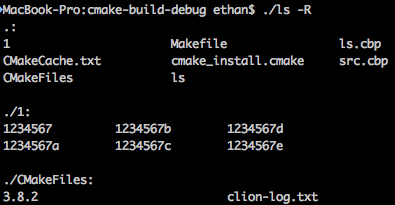
\includegraphics[width=\linewidth]{myls-R}
        \caption{本程序}
      \end{subfigure}
    \caption{本程序和系统的ls命令对比(递归搜索)}
    \label{fig:myls_and_ls_R}
\end{figure}

在不同宽度的窗口中,输出的行数会随之变化。图\ref{fig:myls_width}展示了开启了选项-a、-i,即显示所有文件和inode时,窗口宽度不同本程序的输出。
\begin{figure}[h!]
    \centering
    \begin{subfigure}[b]{0.35\linewidth}
        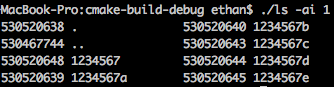
\includegraphics[width=\linewidth]{myls-ai_1_1}
        \caption{窄窗口}
      \end{subfigure}
      \begin{subfigure}[b]{0.55\linewidth}
        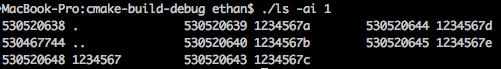
\includegraphics[width=\linewidth]{myls-ai_1_2}
        \caption{宽窗口}
      \end{subfigure}
    \caption{不同宽度下的输出排版}
    \label{fig:myls_width}
\end{figure}

如图\ref{fig:myls_home}所示,输入名称中包含字符\lstinline{'~'}时,会自动替换为Home目录的路径并成功查询。
\begin{figure}[h!]
    \centering
    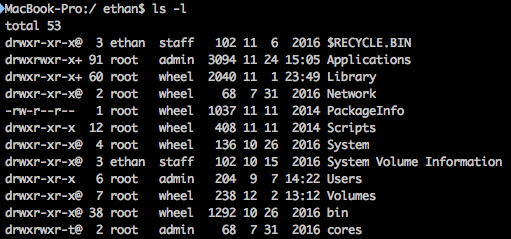
\includegraphics[width=0.7\linewidth]{origin_ls_long_format}
    \caption{输入字符包含\lstinline{'~'}}
    \label{fig:myls_home}
\end{figure}
\newpage

如图\ref{fig:myls_ailrt}所示,程序开启了-a、-i、-l、-r、-t选项,长格式按时间升序显示所有文件,显示inode。
\begin{figure}[h!]
    \centering
    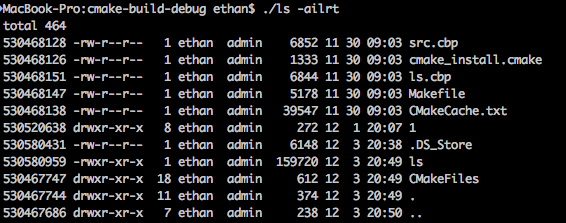
\includegraphics[width=0.7\linewidth]{myls-ailrt}
    \caption{开启选项-ailrt}
    \label{fig:myls_ailrt}
\end{figure}

如图\ref{fig:myls_1}所示,程序开启了-1选项,即无论窗体宽度为多少,都采用单列的方式输出。
\begin{figure}[h!]
    \centering
    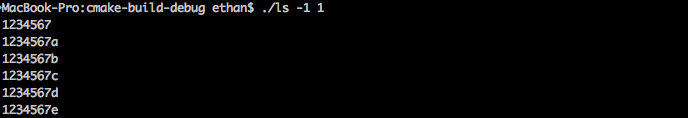
\includegraphics[width=0.7\linewidth]{myls-1}
    \caption{开启选项-1}
    \label{fig:myls_1}
\end{figure}

\newpage
\section{设计体会}

经过本次的大作业,我学会了linux中关于目录和文件的一些系统调用,并且更加巩固了文件、用户、组、文件属性和许可权限的概念。在这次作业的过程中我遇到了许多问题,但是查阅相关网页资料和linux自带的手册后都可以得到解决。本次作业提高了我的实际操作能力,也提高了我编程的能力。实验报告采用 \LaTeX 排版。

\newpage
\printbibliography[heading=bibintoc]

\end{document}